\section{Results}

\subsection{Experimental setting}
The main platform is a Linux virtual machine with 8 virtual processors of an
Intel Core i7-6700 (3.4\,GHz, a processor with 4 cores and 8 hardware threads),
19\,GiB of memory and an NVIDIA Quadro P2000 GPU (5\,GiB, 2017). The software is
Ubuntu 24.04, the GNU Compiler Collection (GCC) 13.3 with \code{-O3 -march=native}, CUDA 12.0, Open MPI 4.1.6
and MPI4Py 4.1.2. A second platform, used for the processor versions only, is
an Apple M4 with 4 performance and 6 efficiency cores and GCC 16.2.

Each configuration runs 2 warm-up repetitions and 7 timed repetitions in one
process, and we report the median. The time covers everything from packets in
host memory to flow records in host memory; for the GPU it includes the upload
and the download. Reading or generating the input is excluded. Large buffers
are recycled between repetitions, as a pipeline that processes one batch after
another would do. Speedup is $S = T_{\mathrm{seq}}/T_{\mathrm{par}}$, measured
against the sequential baseline on the same input, and efficiency is $E = S/p$
for $p$ threads or processes. Unless stated otherwise, synthetic inputs have
$2^{24}$ packets and $2^{20}$ flows.

\subsection{Correctness}
All \nchecks{} checks of the test suite pass on the main platform and all
\nchecksMac{} on the second one. Flow-record accuracy is 100\%: the integer
accumulators of every parallel version are identical to the baseline, and the
largest relative difference in a derived feature is below $10^{-15}$ (the
entropy, which uses a logarithm). The baseline agrees with the independent
Python reference on all its inputs, including the first 60{,}000 packets of the
real trace.

\subsection{Runtime and speedup versus problem size}
Fig.~\ref{fig:size} shows the throughput for $2^{20}$ to $2^{25}$ packets with
moderate skew ($s=1$, $n/16$ flows). At $2^{25}$ packets the baseline needs
3.24\,s (\sizeSeqMpps{} million packets per second). The speedups are
\sizeChunkSp\x{} for \code{gpu-chunk}, \sizePartSp\x{} for \code{omp-part},
\sizeAtomicSp\x{} for \code{gpu-atomic}, \sizeFlowSp\x{} for \code{gpu-flow} and
\sizeMergeSp\x{} for \code{omp-merge}. The baseline slows down as the batch
grows, from \sizeSeqSmallMpps{} to \sizeSeqMpps{} million packets per second,
because its table stops fitting in the cache. The partitioned and GPU
versions keep an almost constant throughput, so their speedup grows with the
problem size.

\begin{figure}[H]
\centering
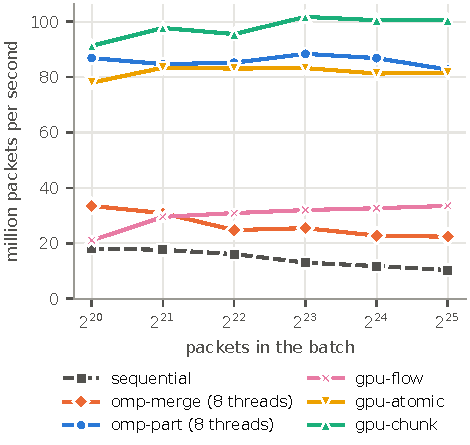
\includegraphics[width=\linewidth]{throughput_vs_size.pdf}
\caption{Throughput versus batch size on synthetic traffic ($s=1$). OpenMP
versions use 8 threads. Higher is better.}
\label{fig:size}
\end{figure}

\subsection{Effect of skew and of the number of flows}
Table~\ref{tab:skew} and Fig.~\ref{fig:skew} vary the Zipf exponent. Three
effects appear.

First, skew helps the baseline: it is \skewSeqRatio\x{} faster at $s=2$ than at
$s=0$, because the popular records stay in the cache. Table~\ref{tab:flows}
isolates this effect with uniform traffic: the baseline costs
\flowsSeqNsSmall\,ns per packet with 256 flows and \flowsSeqNsBig\,ns with 4
million flows.

Second, the two OpenMP strategies react in opposite ways. \code{omp-part} is
\skewPartSpZero\x{} faster than the baseline at $s=0$ but only
\skewPartSpTwo\x{} at $s=2$: the largest flow has \topshareTwo\% of the packets
and its partition is processed by one thread. \code{omp-merge} is weak with
many flows (\skewMergeSpZero\x{} at $s=0$), because every thread builds a table
almost as large as the global one and the merge repeats the work, and it is
the best processor version under heavy skew (\skewMergeSpHi\x{} at $s=1.5$).

Third, on the GPU the kernel with one thread per flow is the fastest for
uniform traffic and collapses with skew: at $s=2$ it is \skewFlowSlow\x{}
slower than \code{gpu-chunk} and 12 times slower than the baseline, because
one GPU thread walks 10 million packets. \code{gpu-atomic} is stable, and
\code{gpu-chunk} is the best or close to the best for every $s \ge 0.8$.

\begin{table}[H]
\centering\footnotesize
\setlength{\tabcolsep}{3.2pt}
\caption{Runtime in milliseconds versus Zipf exponent $s$ ($2^{24}$ packets).
The best time of each column is in bold.}\label{tab:skew}
\begin{tabular}{@{}l rrrrrrr@{}}
\toprule
$s$ & 0 & 0.5 & 0.8 & 1.0 & 1.2 & 1.5 & 2.0 \\
\midrule
\tabinput{tables/skew_short.tex}
\bottomrule
\end{tabular}
\end{table}

\begin{figure}[H]
\centering
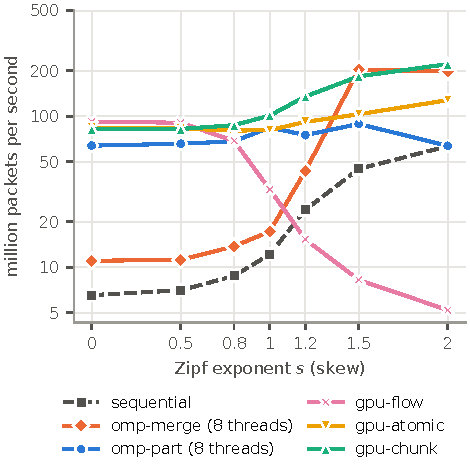
\includegraphics[width=\linewidth]{throughput_vs_skew.pdf}
\caption{Throughput versus skew (logarithmic vertical axis), same runs as
Table~\ref{tab:skew}.}
\label{fig:skew}
\end{figure}

\begin{table}[H]
\centering\footnotesize
\setlength{\tabcolsep}{4pt}
\caption{Runtime in milliseconds versus number of flows (uniform traffic,
$2^{24}$ packets). Best time per column in bold.}\label{tab:flows}
\begin{tabular}{@{}l rrrrrr@{}}
\toprule
Flows & $2^{8}$ & $2^{12}$ & $2^{16}$ & $2^{18}$ & $2^{20}$ & $2^{22}$ \\
\midrule
\tabinput{tables/flows.tex}
\bottomrule
\end{tabular}
\end{table}

\subsection{Strong and weak scaling with OpenMP}
Fig.~\ref{fig:scaling}(a,b) and Table~\ref{tab:strong} show strong scaling.
For \code{omp-part} at $s=0$ the speedup over the baseline is
\ssPartZeroFour\x{} with 4 threads, an efficiency above 100\%. This is not only
parallelism: with one thread the partitioned algorithm is already
\ssPartZeroOne\x{} faster than the baseline because each partition fits in the
cache. Against its own one-thread time, 4 threads give \ssPartZeroSelfFour\x{}
and 8 threads \ssPartZeroSelf\x. The curves flatten after 4 threads
because the machine has 4 physical cores. At $s=1.5$ the load imbalance limits
\code{omp-part} to \ssPartHiEight\x, while \code{omp-merge} reaches
\ssMergeHiEight\x{} (\ssMergeHiSelf\x{} against its own one-thread time).

\begin{figure*}[t]
\centering
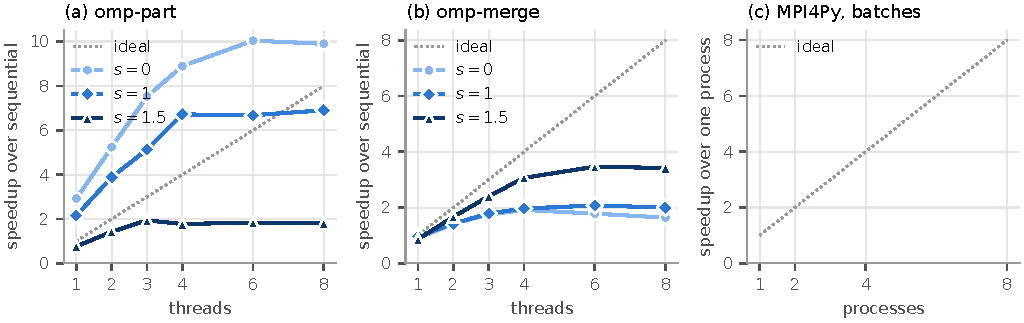
\includegraphics[width=\linewidth]{scaling.pdf}
\caption{Strong scaling. (a), (b): speedup of the two OpenMP strategies over
the sequential baseline for three skews ($2^{24}$ packets). (c): speedup of the
MPI4Py driver over one process, for 30 real batches and for 16 synthetic
batches of uneven size, with static and dynamic schedules. The dotted line is
the ideal speedup.}
\label{fig:scaling}
\end{figure*}

\begin{table}[H]
\centering\footnotesize
\setlength{\tabcolsep}{3.4pt}
\caption{Strong scaling on the main platform. $T_{\mathrm{seq}}$ in
milliseconds; speedup over the baseline with 1 to 8 threads; $E_8$ is the
efficiency with 8 threads; ``self'' is the speedup of 8 threads over 1 thread
of the same strategy.}\label{tab:strong}
\begin{tabular}{@{}l r r rrrr r r@{}}
\toprule
 & $s$ & $T_{\mathrm{seq}}$ & 1 & 2 & 4 & 8 & $E_8$ & self \\
\midrule
\tabinput{tables/strong.tex}
\bottomrule
\end{tabular}
\end{table}

For weak scaling (Table~\ref{tab:weak}) the input grows with the thread
count, $2^{22}$ packets and $2^{18}$ flows per thread. Efficiency falls to
\weakPartEff\% for \code{omp-part} and \weakMergeEff\% for \code{omp-merge} at
8 threads. Two causes add up: only 4 cores are available, and the cost per
packet itself grows with the number of flows (the baseline takes 11 times
longer for 8 times more data).

\begin{table}[H]
\centering\footnotesize
\setlength{\tabcolsep}{3.6pt}
\caption{Weak scaling ($s=1$): runtime in milliseconds and efficiency
$T(1)/T(p)$ of each strategy.}\label{tab:weak}
\begin{tabular}{@{}r r r rr rr@{}}
\toprule
 & & & \multicolumn{2}{c}{omp-part} & \multicolumn{2}{c}{omp-merge} \\
Threads & Packets & seq & time & eff. & time & eff. \\
\midrule
\tabinput{tables/weak.tex}
\bottomrule
\end{tabular}
\end{table}

Table~\ref{tab:mac} repeats the experiment on the Apple M4, including the
one-minute real batch. The pattern is the same, and the programs scale
further: \code{omp-part} reaches \macPartZeroTen\x{} over the baseline with 10
threads at $s=0$, and \code{omp-merge} reaches \macMergeHiTen\x{} at $s=1.5$.
Gains are smaller beyond 4 threads, where the efficiency cores come into use.

\begin{table}[H]
\centering\footnotesize
\setlength{\tabcolsep}{3pt}
\caption{Second platform (Apple M4): $T_{\mathrm{seq}}$ in milliseconds and
speedup over the baseline with 1 to 10 threads, for synthetic traffic and for
the one-minute real batch.}\label{tab:mac}
\begin{tabular}{@{}l r r rrrrrr@{}}
\toprule
 & $s$ & $T_{\mathrm{seq}}$ & 1 & 2 & 4 & 6 & 8 & 10 \\
\midrule
\tabinput{tables/mac.tex}
\bottomrule
\end{tabular}
\end{table}

\subsection{Contention on a shared table}\label{sec:contention}
Fig.~\ref{fig:contention} shows the micro-benchmark that motivates avoiding a
shared table. It computes only the order-independent features. With uniform
traffic, 8 threads on a shared table are \contLockZero\x{} (locks) and
\contAtomicZero\x{} (atomics) faster than one thread. At $s=1.5$ the shared
table with locks drops to \contLockHiMpps{} million packets per second, 3 times
\emph{slower} than one thread (\contSeqHi{} million), and at $s=2$ it is
\contLockTwo{} times slower: the threads take turns on the record of the
largest flow and its cache line moves between cores on every update. Private
tables with a merge reach \contLocalHiMpps{} million packets per second at
$s=1.5$.

\begin{figure}[H]
\centering
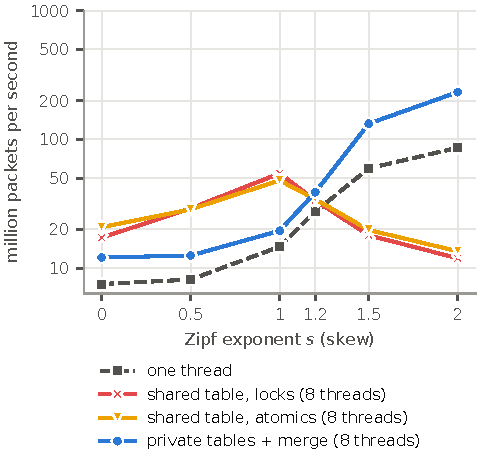
\includegraphics[width=\linewidth]{contention.pdf}
\caption{Shared hash table under skew: throughput of the order-independent
aggregation ($2^{24}$ packets, $2^{18}$ flows, logarithmic axis).}
\label{fig:contention}
\end{figure}

\subsection{GPU: time breakdown, transfers and launch configuration}
Fig.~\ref{fig:gpu} splits the time of \code{gpu-chunk}. For synthetic traffic
at $s=1$, grouping takes \gpuOneGroupShare\% and the two transfers
\gpuOneXferShare\%. For the real trace the download alone takes
\gpuRealDownShare\%: the batch is \xferRealInMB\,MB of packets but produces
\xferRealOutMB\,MB of records, because it has 3.2 million flows of 248 bytes
each.

\begin{figure}[H]
\centering
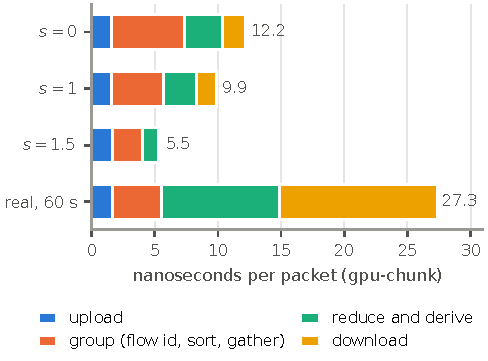
\includegraphics[width=\linewidth]{gpu_breakdown.pdf}
\caption{Time of \code{gpu-chunk} per packet, by stage. The number at the end
of each bar is the total in nanoseconds per packet.}
\label{fig:gpu}
\end{figure}

\emph{Memory transfers.} Uploading from page-locked host memory reaches
\xferUpPinDirect\,GB/s against \xferUpPageDirect\,GB/s from pageable memory.
For the download, copying directly into the recycled result buffer
(\xferDownPinDirect\,GB/s) is faster than downloading into page-locked memory
and copying again (\xferDownPinStaged\,GB/s). The best combination processes
the real batch in \xferTotalPinDirect\,ms and the worst in
\xferTotalPageStaged\,ms.

\emph{Launch configuration.} Table~\ref{tab:gpucfg} shows that the number of
threads per block matters little: the kernels are simple maps limited by
memory, and the spread is \tpbSpreadAtomic\% for \code{gpu-atomic} and
\tpbSpreadChunk\% for \code{gpu-chunk}. The chunk size matters a lot. With one
packet per thread and $s=1.5$ the reduction takes \chunkHiOne\,ms, because
thousands of threads update the same record atomically. With 8 packets per
thread it takes \chunkHiBest\,ms. Larger chunks are slower again
(\chunkHiLast\,ms at 255) because each thread then reads a long private range
and neighboring threads no longer touch neighboring memory. We use 8 as the
default.

\begin{table}[H]
\centering\footnotesize
\setlength{\tabcolsep}{2.6pt}
\caption{GPU launch configuration, times in milliseconds, best per row in
bold. Top: total time versus threads per block ($s=1$). Bottom: time of the
reduction stage of \code{gpu-chunk} versus packets per thread.}\label{tab:gpucfg}
\begin{tabular}{@{}l rrrrrr@{}}
\toprule
Threads per block & 32 & 64 & 128 & 256 & 512 & 1024 \\
\midrule
\tabinput{tables/gpu_tpb.tex}
\bottomrule
\end{tabular}

\vspace{4pt}
\begin{tabular}{@{}l rrrrrrrrr@{}}
\toprule
Chunk & 1 & 2 & 4 & 8 & 16 & 32 & 64 & 128 & 255 \\
\midrule
\tabinput{tables/gpu_chunk.tex}
\bottomrule
\end{tabular}
\end{table}

\subsection{Real backbone traffic}
Table~\ref{tab:real} gives the results on the real trace. In one minute,
\realSingle\% of the flows have a single packet, and \realHalfFlows{} flows
(\realHalfPct\% of them) carry half of the packets. The three GPU kernels are
equivalent here, about 4.3\x{} faster than the baseline (\realChunkMpps{}
million packets per second), and the speedup holds up to the largest batch
that fits in the 5\,GiB of the GPU. \code{omp-part} reaches \realPartSp\x{} and
\code{omp-merge} \realMergeSp\x. The gains are smaller than on synthetic
traffic because there is one record for every 2.4 packets: producing 789\,MB
of output is a large part of the work for every version.

On the Apple M4 (Table~\ref{tab:mac}) the baseline processes the one-minute
batch in \macRealSeq\,ms (\macRealSeqMpps{} million packets per second) and
\code{omp-part} is \macRealPartBest\x{} faster with 8 threads. That is
81\,ms, less than the \xferTotalPinDirect\,ms of the GPU pipeline on the
main platform: a current processor with the partitioned algorithm outruns
this 2017 GPU on mice-dominated traffic.

\begin{table}[H]
\centering\footnotesize
\setlength{\tabcolsep}{3.4pt}
\caption{Real trace: runtime in milliseconds and speedup over the baseline
for batches of 60, 120 and 240 seconds. OpenMP versions use 8 threads. Best
speedup per batch in bold.}\label{tab:real}
\begin{tabular}{@{}l rr rr rr@{}}
\toprule
 & \multicolumn{2}{c}{60 s} & \multicolumn{2}{c}{120 s} & \multicolumn{2}{c}{240 s} \\
 & ms & $S$ & ms & $S$ & ms & $S$ \\
\midrule
\tabinput{tables/real.tex}
\bottomrule
\end{tabular}
\end{table}

\subsection{Distributed batches with MPI4Py}
The 15-minute trace was cut into 30 batches of 30 seconds
(\mpiPackets{} million packets, \mpiFlows{} million flow records in total).
Table~\ref{tab:mpi} and Fig.~\ref{fig:scaling}(c) show the results with the
sequential kernel in every process. One process needs \mpiOneWall\,s. With 4
processes the speedup is \mpiStaticSpFour\x, and with 8 it is only
\mpiStaticSp\x{} (efficiency \mpiStaticEff\%). The cause is not communication:
the summaries are tiny and the shared counter of the dynamic schedule costs
\mpiSchedMs\,ms in total. The kernel is limited by memory. When we run
independent copies of the sequential program on one batch, each copy takes
0.50\,s alone, 0.81\,s with 4 copies and 1.53\,s with 8 copies. The same test
on an input that fits in the cache takes 0.23\,s alone, 0.24\,s with 4 copies
and 0.56\,s with 8, which is the effect of having 4 physical cores.

\begin{table}[H]
\centering\footnotesize
\setlength{\tabcolsep}{3pt}
\caption{MPI4Py strong scaling: wall time in seconds and speedup $S$ over one
process, for the real batches and for the batches of uneven size.}\label{tab:mpi}
\begin{tabular}{@{}r rr rr rr rr@{}}
\toprule
 & \multicolumn{4}{c}{30 real batches} & \multicolumn{4}{c}{16 uneven batches} \\
 & \multicolumn{2}{c}{static} & \multicolumn{2}{c}{dynamic} & \multicolumn{2}{c}{static} & \multicolumn{2}{c}{dynamic} \\
$p$ & s & $S$ & s & $S$ & s & $S$ & s & $S$ \\
\midrule
\tabinput{tables/mpi.tex}
\bottomrule
\end{tabular}
\end{table}

\emph{Load balance.} The real batches have similar sizes, so static and
dynamic schedules perform the same. The uneven set has two batches of
$2^{24}$ packets followed by fourteen of $2^{21}$. With 4 processes the static
schedule gives both large batches to process 0 and reaches
\mpiUnevenStaticSpFour\x, while the dynamic schedule reaches
\mpiUnevenDynSpFour\x. With 8 processes on 4 cores both become slower than
with 4.

\emph{Other measurements.} In weak scaling (3 real batches per process) the
efficiency is \mpiWeakEff\% at 8 processes, for the same memory reason.
Collecting all flow records at process 0 instead of summaries is expensive:
for 8 batches (\mpiCollectGB\,GB of records) and 8 processes the wall time
grows \mpiCollectSlow\x{} and the collection takes \mpiCollectShare\% of it. A
real deployment should write the records where they are produced. Finally,
combining both models, 2 processes with 4 threads of \code{omp-part} each
process the whole trace in \mpiHybridBestS\,s (\mpiHybridBestMpps{} million
packets per second), \mpiHybridSp\x{} faster than one sequential process.
